\documentclass[a4paper,11pt]{article}
%Premeable
	%Chinese
	\usepackage[UTF8,fontset=fandol]{ctex}
	\usepackage{xeCJK}
	\usepackage[datesep=/]{datetime2}
	\DeclareTextFontCommand{\textbf}{\sffamily}
%Presenting
	\usepackage[table]{xcolor}
	\usepackage{graphicx}
	\usepackage[font={sf}]{caption}
	\usepackage[above]{placeins}
	\usepackage{float,wrapfig}
	\usepackage{tabularx,array,booktabs,multirow,bigstrut}
	\newcolumntype{C}[1]{>{\hsize=#1\hsize%
		\centering\arraybackslash}X}
	\newcommand{\minitab}[2][l]{%
		\begin{tabular}{#1}#2\end{tabular}}
%MathSetting
	\let\latexointop\ointop
	\usepackage{amsmath,bm,amssymb,esint,extarrows}
	\usepackage{upgreek,textcomp,mathrsfs}
	\usepackage[only,sslash]{stmaryrd}
	\usepackage{nicefrac,eqnarray}
%	\usepackage{amsthm}
	\usepackage{mathtools,physics,siunitx}
	\usepackage{stackengine,titling,varwidth}
	\usepackage{tikz}
	\usepackage{resizegather,empheq}
	\usetagform{default}
	\usepackage{calligra,fourier-orns}
	% Keep \oint unchanged by esint
	\let\ointop\undefined
	\let\ointop\latexointop
	% Define a scriptr 
	\DeclareMathAlphabet{\mathcalligra}{T1}{calligra}{m}{n}
	\DeclareFontShape{T1}{calligra}{m}{n}{<->s*[2.2]callig15}{}
	\newcommand{\scriptr}{\mathcalligra{r}\,}
	\newcommand{\rvector}{\pmb{\mathcalligra{r}}\,}
	% Useful shorthand
	\DeclarePairedDelimiter\ave{\langle}{\rangle}
	\newcommand\inlineeqno{\stepcounter{equation}\ (\theequation)}
	\newcommand{\sinc}{\operatorname{sinc}}
	\newcommand{\mbb}[1]{\mathbb{#1}}
	\newcommand{\mrm}[1]{\mathrm{#1}}
	\newcommand{\mcal}[1]{\mathcal{#1}}
	% Scaling and positioning
	\newcommand\scalemath[2]{\scalebox{#1}{\mbox{\ensuremath{\displaystyle #2}}}}
	\newcommand\raisemath[2]{\raisebox{#1\depth}{${#2}$}}
	\empheqset{box=\bbox}
	% Presenting
	\newcommand*\bbox[1]{\fbox{\hspace{1em}\addstackgap[5pt]{#1}\hspace{1em}}}
	\sisetup{%
		redefine-symbols=false,%
		separate-uncertainty=true,%
		range-phrase=\,\textasciitilde\,,%
		arc-separator = \,}
	\allowdisplaybreaks[2]
%ParagraphSetting
	\setlength{\parskip}{.3\baselineskip}
	\usepackage[defaultlines=2,all]{nowidow}
	\postdisplaypenalty=50
%PageSetting
	\usepackage[colorlinks=true,linkcolor=blue]{hyperref}
	\usepackage[vmargin={4cm,5cm},hmargin=3cm,%
		footnotesep=\baselineskip]{geometry}
	\usepackage[bottom]{footmisc}
	\usepackage{changepage}
	% Autoref names
	\renewcommand{\tableautorefname}{\tablename}
	\renewcommand{\figureautorefname}{\figurename}
	% List settings
	\usepackage{enumitem}
	\setlist{itemsep=0pt,topsep=0pt,labelindent=\parindent,leftmargin=0pt,itemindent=*}
	% Some redefined lengths
	\setlength{\headsep}{2.2cm}
	\setlength{\droptitle}{-2.2cm}
	\setlength{\footnotesep}{3\parskip}
	% Header
	\usepackage{fancyhdr,lastpage}
	\pagestyle{fancy}
	\fancyhf{}
	\cfoot{--\ \thepage\,/\,\pageref{LastPage} \ --}
	\renewcommand{\headrulewidth}{0.1pt}
	\renewcommand{\headrule}{
		\vbox to 2pt{
		\hbox to \headwidth{\dotfill}\vss}}
	% Separator
	\newcommand{\newparagraph}{\pagebreak[3]\noindent%
		\hfil
		~\raisebox{-4pt}[10pt][10pt]{\decofourright~~~~~~~~\decofourleft}~ %
		\par
	}
%TitleSettings
	\pretitle{\begin{center}}
	\posttitle{\par\end{center}\vspace{-6mm}}
	\predate{}
	\postdate{\vspace{-4mm}}
%Header
	\lhead{%
		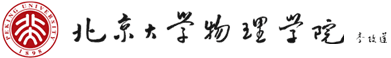
\includegraphics[height=3.2em]{PKUPhy.png}
		\vspace{-3ex}
		}
	\rhead{%
		\itshape\small
		\begin{tabular}{rr}
			\multicolumn{2}{r}{赵启渊} \\[.3em]
			学号:   & 2000011153 \\[.2em]
		\end{tabular}\hspace{-1em}
		}
%Title
	\title{\textit{\large 实验十二}\\[2mm]
		\textbf{\LARGE 测量介质中的声速}}
	\author{\textit{赵启渊} 2000011153}
	\date{}
%Miscellaneous
	\newcommand{\tabindent}{\hspace{2em}}
%FourierTransform
	\newcommand{\ftransform}{\xlongrightarrow{\ \mathscr F\ }}
	\newcommand{\iftransform}{\xlongrightarrow{\ \mathscr F^{-1}\ }}
	\usepackage{gensymb}

\begin{document}
	
	
\maketitle
\thispagestyle{fancy}
\begin{enumerate}
	\item 极值法(共振干涉法、驻波法)和相位法(李萨如图形、行波法)测定空气中的声速分别是什么原理?\\
	解:因为有公式$ v = f * \lambda $,在频率已知的情况下,只需要测定波长即可。\\
	极值法:声波在空气中传播遇到一刚性平面时会反射回来,反射声波和入射声波发生干涉,形成驻波。在驻波场中,坐标为x的空气质点,位移$\xi$有$$ \xi = \dfrac{a\sin[k(l-x)]}{\sin kl}\cos \omega t $$
	$$ k = \frac{2*\pi}{\lambda} = \frac{\omega}{v}$$
	k是波数,l是声源和平面之间的距离。驻波有波腹和波节,两个相邻波腹波节之间距离是$\frac{\lambda}{2}$.我们通过测量声压来反映位移驻波,根据声学理论有$$ p = \rho_0 \omega v \dfrac{a\sin[k(l-x)+\frac{\pi}{2}]}{\sin kl}\cos \omega t $$
	位移驻波为波腹时,声压为波节;位移驻波为波节时,声压为波腹。刚平面处有关系$$ |p(l \pm \frac{\lambda}{2} )| = |p(l)| $$我们读出刚平面处的声压振幅大小,根据$ |p(l)| $随l变化的关系,就可以求出$\frac{\lambda}{2}$,从而求出声速。 \\
	行波法:行波位移$\xi$有$$ \xi = a\cos (\omega t- kx) $$
	$$ k = \frac{2*\pi}{\lambda} = \frac{\omega}{v}$$
	根据声学的公式有$$ p(0) = - \rho_0 v \omega a \sin \omega t $$
	$$ p(l) = - \rho_0 v \omega a \sin (\omega t - kl) $$
    他们相位差是kl。利用示波器接相对应的声源处和接收器处的电压信号,可以观察到李萨如图形,调节l,使得图形恢复原状,l就等于$\lambda$,从而测出波长和声速。	
	
	\item 由信号源直接输入示波器的信号在极值法和相位法中分别有什么作用? \\
	解:极值法:确定信号发生器发生稳定,大小适当的声波,并且使得频率为谐振频率,提高监测灵敏度。\\
	相位法:作为其中一个参数形成李萨如图形。
	
	\item 如何将换能器调节到工作在共振频率?\\
	解:调节信号发生器和示波器,先使得示波器有稳定,大小适当的波形。调节信号发生器频率,微微改变接收端位置,使正弦波有最大振幅,此时满足题意。
	\item 极值法和相位法测量过程中如何避免声速测定仪回程差(如螺距差)的影响?\\
	解:缓慢转动手轮,尽量避免回转,如果实在要回转的时候,先回转1圈以上,再继续进行测量,从而尽量避免回程差带来的误
	差。
	\item 了解温度计、湿度计和水银气压计的工作原理,分别简述其在测量过程中需要注意的问题。\\
	解:水银气压计:注意水银凸面的形状,可用手指轻轻弹动,使得其正常;注意示数的读取的方法要标准;要保证象牙针G和倒影刚刚接触;注意温度、重力加速度、毛细作用导致水银面降低的修正。\\
	温度计:要等待温度计的示数稳定后再读数;读温度计示数时眼睛要平视。\\
	湿度计:所处环境不应有剧烈的空气流动;注意不应使得细纱布被污染,从而使湿球的平衡温度发生漂移,干湿差变小;应用专用纱套,湿球纱套出了吸水性能外,在厚度上也有要求;读温度计示数时眼睛要平视。
	\item 从介质角度出发,水中声速的测定与空气中相比要有哪些特殊考虑?\\
	解:水的黏滞性和密度比空气都较大,在空气中可以观察到的双峰现象在水中可能不明显。 
	\item 用第一种方法,为什么要在正弦波幅度为极大时进行测量?用第二种方法时,为什么要在李萨如图形呈直线的时候测量?\\
	解: 极值法中,极大值要比极小值明显,人眼更容易判断,提高了判断的精度,所以要用极大值进行测量。\\
	行波法中,李萨如图形呈直线的时候人眼更容易判断,提高了判断的精度。  
\end{enumerate}



	\vfill\noindent\itshape\footnotesize
	\hfill Last edited: \today\ \copyright\ 赵启渊
\end{document}